\chapter{Polarizacion de la Juntura B-E}
    La \textbf{juntura base-emisor (BE)} del transistor BJT es una unión PN que debe estar \textit{polarizada en directa} para que el dispositivo opere en la región activa, es decir, como amplificador. Al aplicar una tensión positiva entre base y emisor (en un transistor NPN), los portadores mayoritarios pueden cruzar la barrera de potencial, permitiendo el flujo de corriente.
    
    Cuando la juntura BE se encuentra polarizada directamente:
    
    \[
    V_{BE} \approx 0.6\,\text{V} \text{ a } 0.7\,\text{V} \quad \text{(para transistores de silicio)}
    \]
    
    Bajo esta condición:
    \begin{itemize}
        \item Se establece una corriente de base $I_B$, que controla el valor de la corriente de colector $I_C$.
        \item Se cumple la relación característica:
        \[
        I_C = \beta \cdot I_B
        \]
        donde $\beta$ es la ganancia de corriente en configuración emisor común.
    \end{itemize}
    
    El análisis de la polarización de la juntura BE permite determinar en qué región de operación se encuentra el transistor (corte, activa o saturación) y es fundamental para comprender su comportamiento tanto en circuitos amplificadores como en aplicaciones digitales. En este trabajo práctico se estudiará experimentalmente la relación entre $V_{BE}$ e $I_B$, obteniendo la característica de la unión base-emisor.

\newpage

  \section{Simulacion}

    Se pide simular para observar la curva de la corriente de base a medida que aumenta la tensión de polarización de la juntura base-emisor, de esta forma poder visualizar el codo de la corriente y la estabilidad de la tension $V_{BE}$ una vez polarizada la juntura.

    %Circuito utilizado en el simulador
    %Grafico de la curva del simulador
    

    

\newpage

    
  \section{Laboratorio}


    Se pide realizar el mismo circuito implementado en la simulacion para poder ver su comportamiento cuando se polariza el transisto, a continuacion se presenta una imagen del circuito implementado en el laboratorio:\\


    \begin{figure}[!ht]

        \begin{minipage}{0.5\textwidth}
            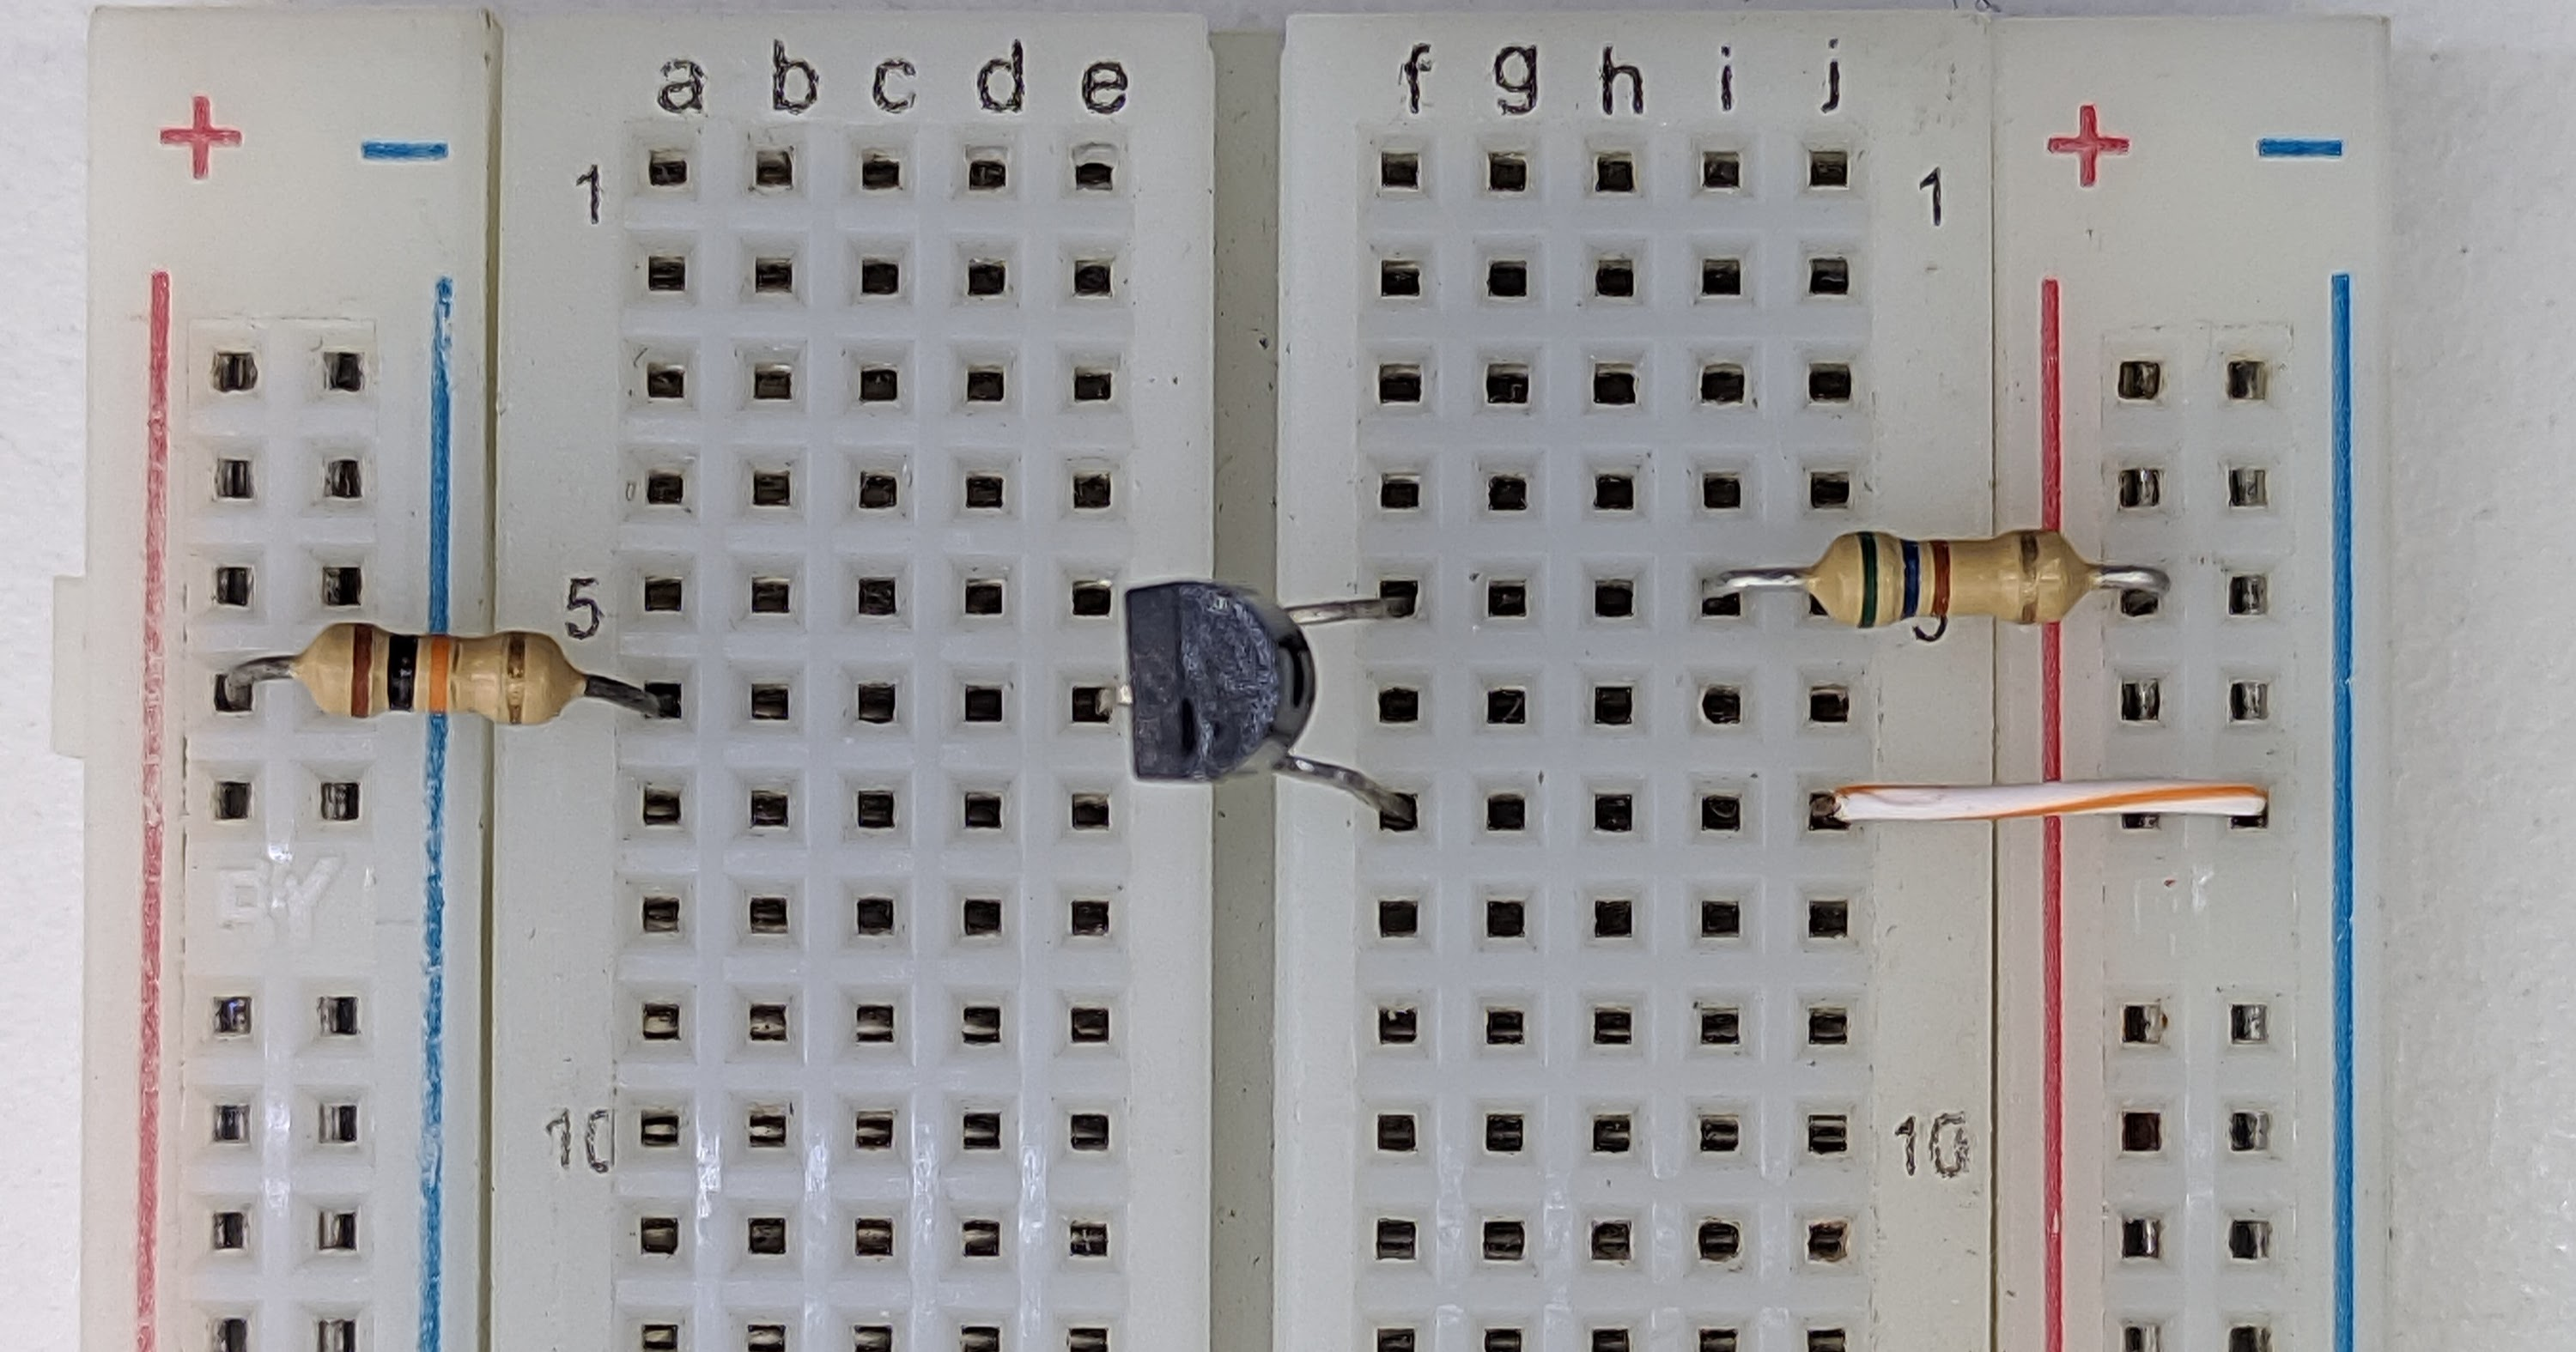
\includegraphics[width=1\textwidth]{tp3/pictures/prot_crkt-1.jpg}
            \caption{Circuito implementado.}
 
        \end{minipage}
                    \begin{minipage}{0.5\textwidth}
            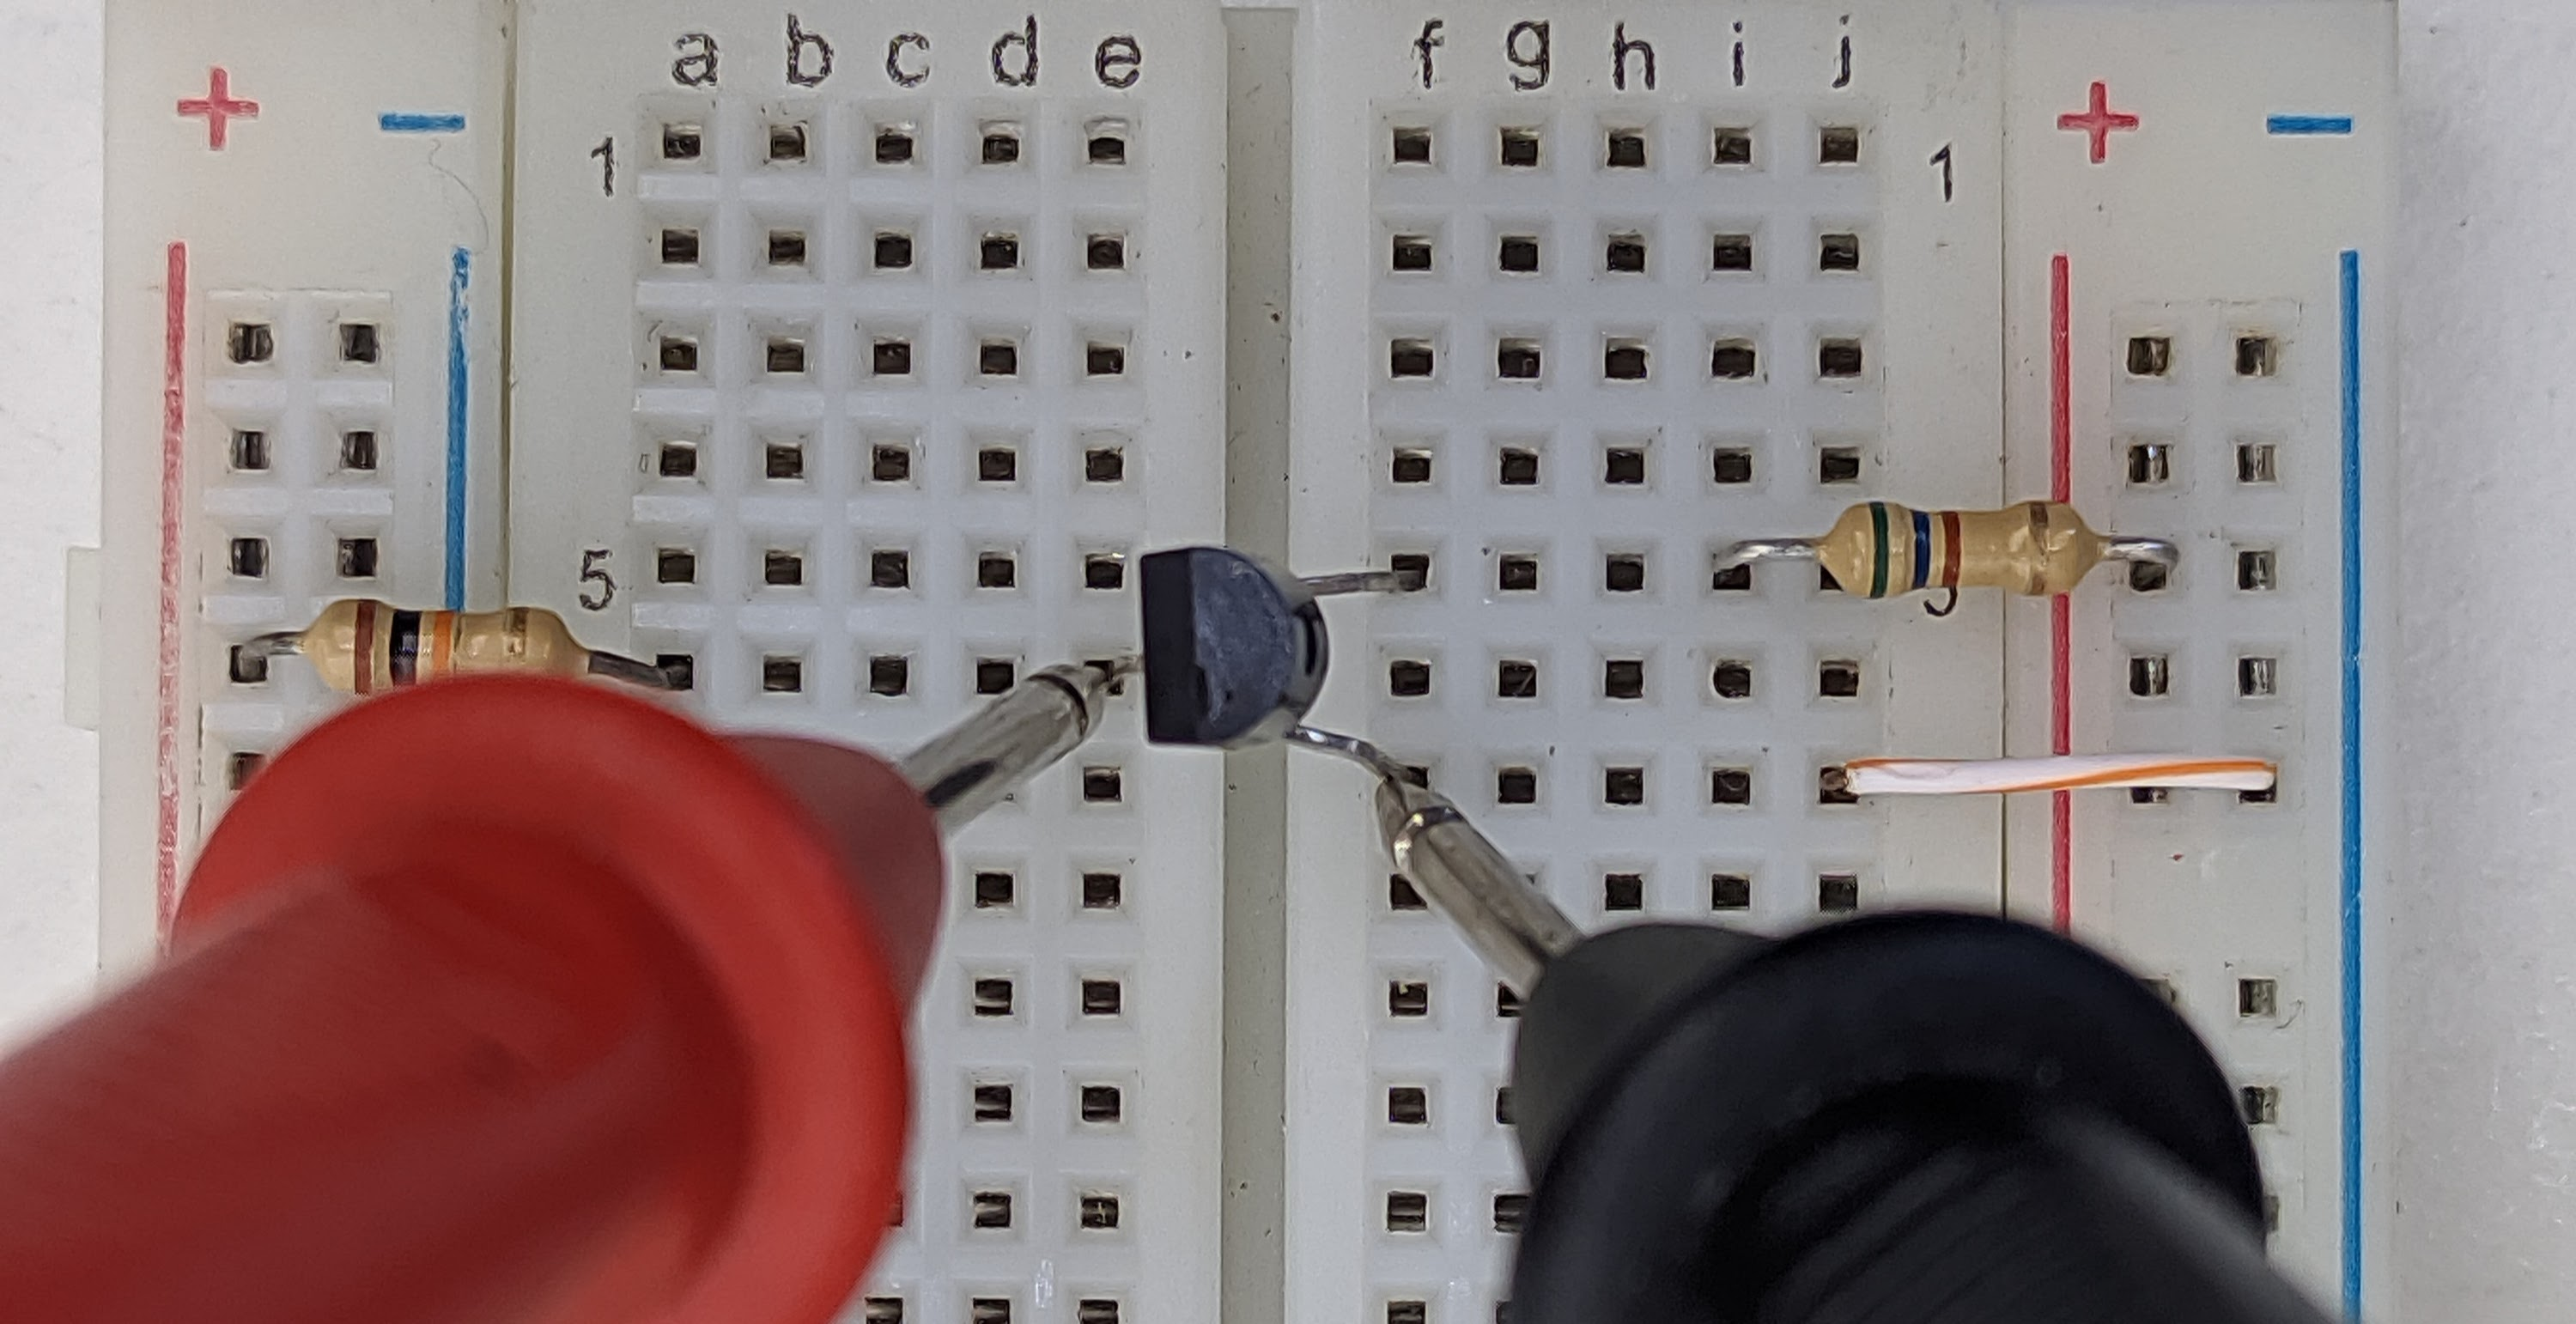
\includegraphics[width=1\textwidth]{tp3/pictures/prot_crkt-1_Vbe.jpg}
            \caption{Medicion de $V_{be}$.}

        \end{minipage}
        
        \begin{center}
         \begin{minipage}{0.5\textwidth}
        
            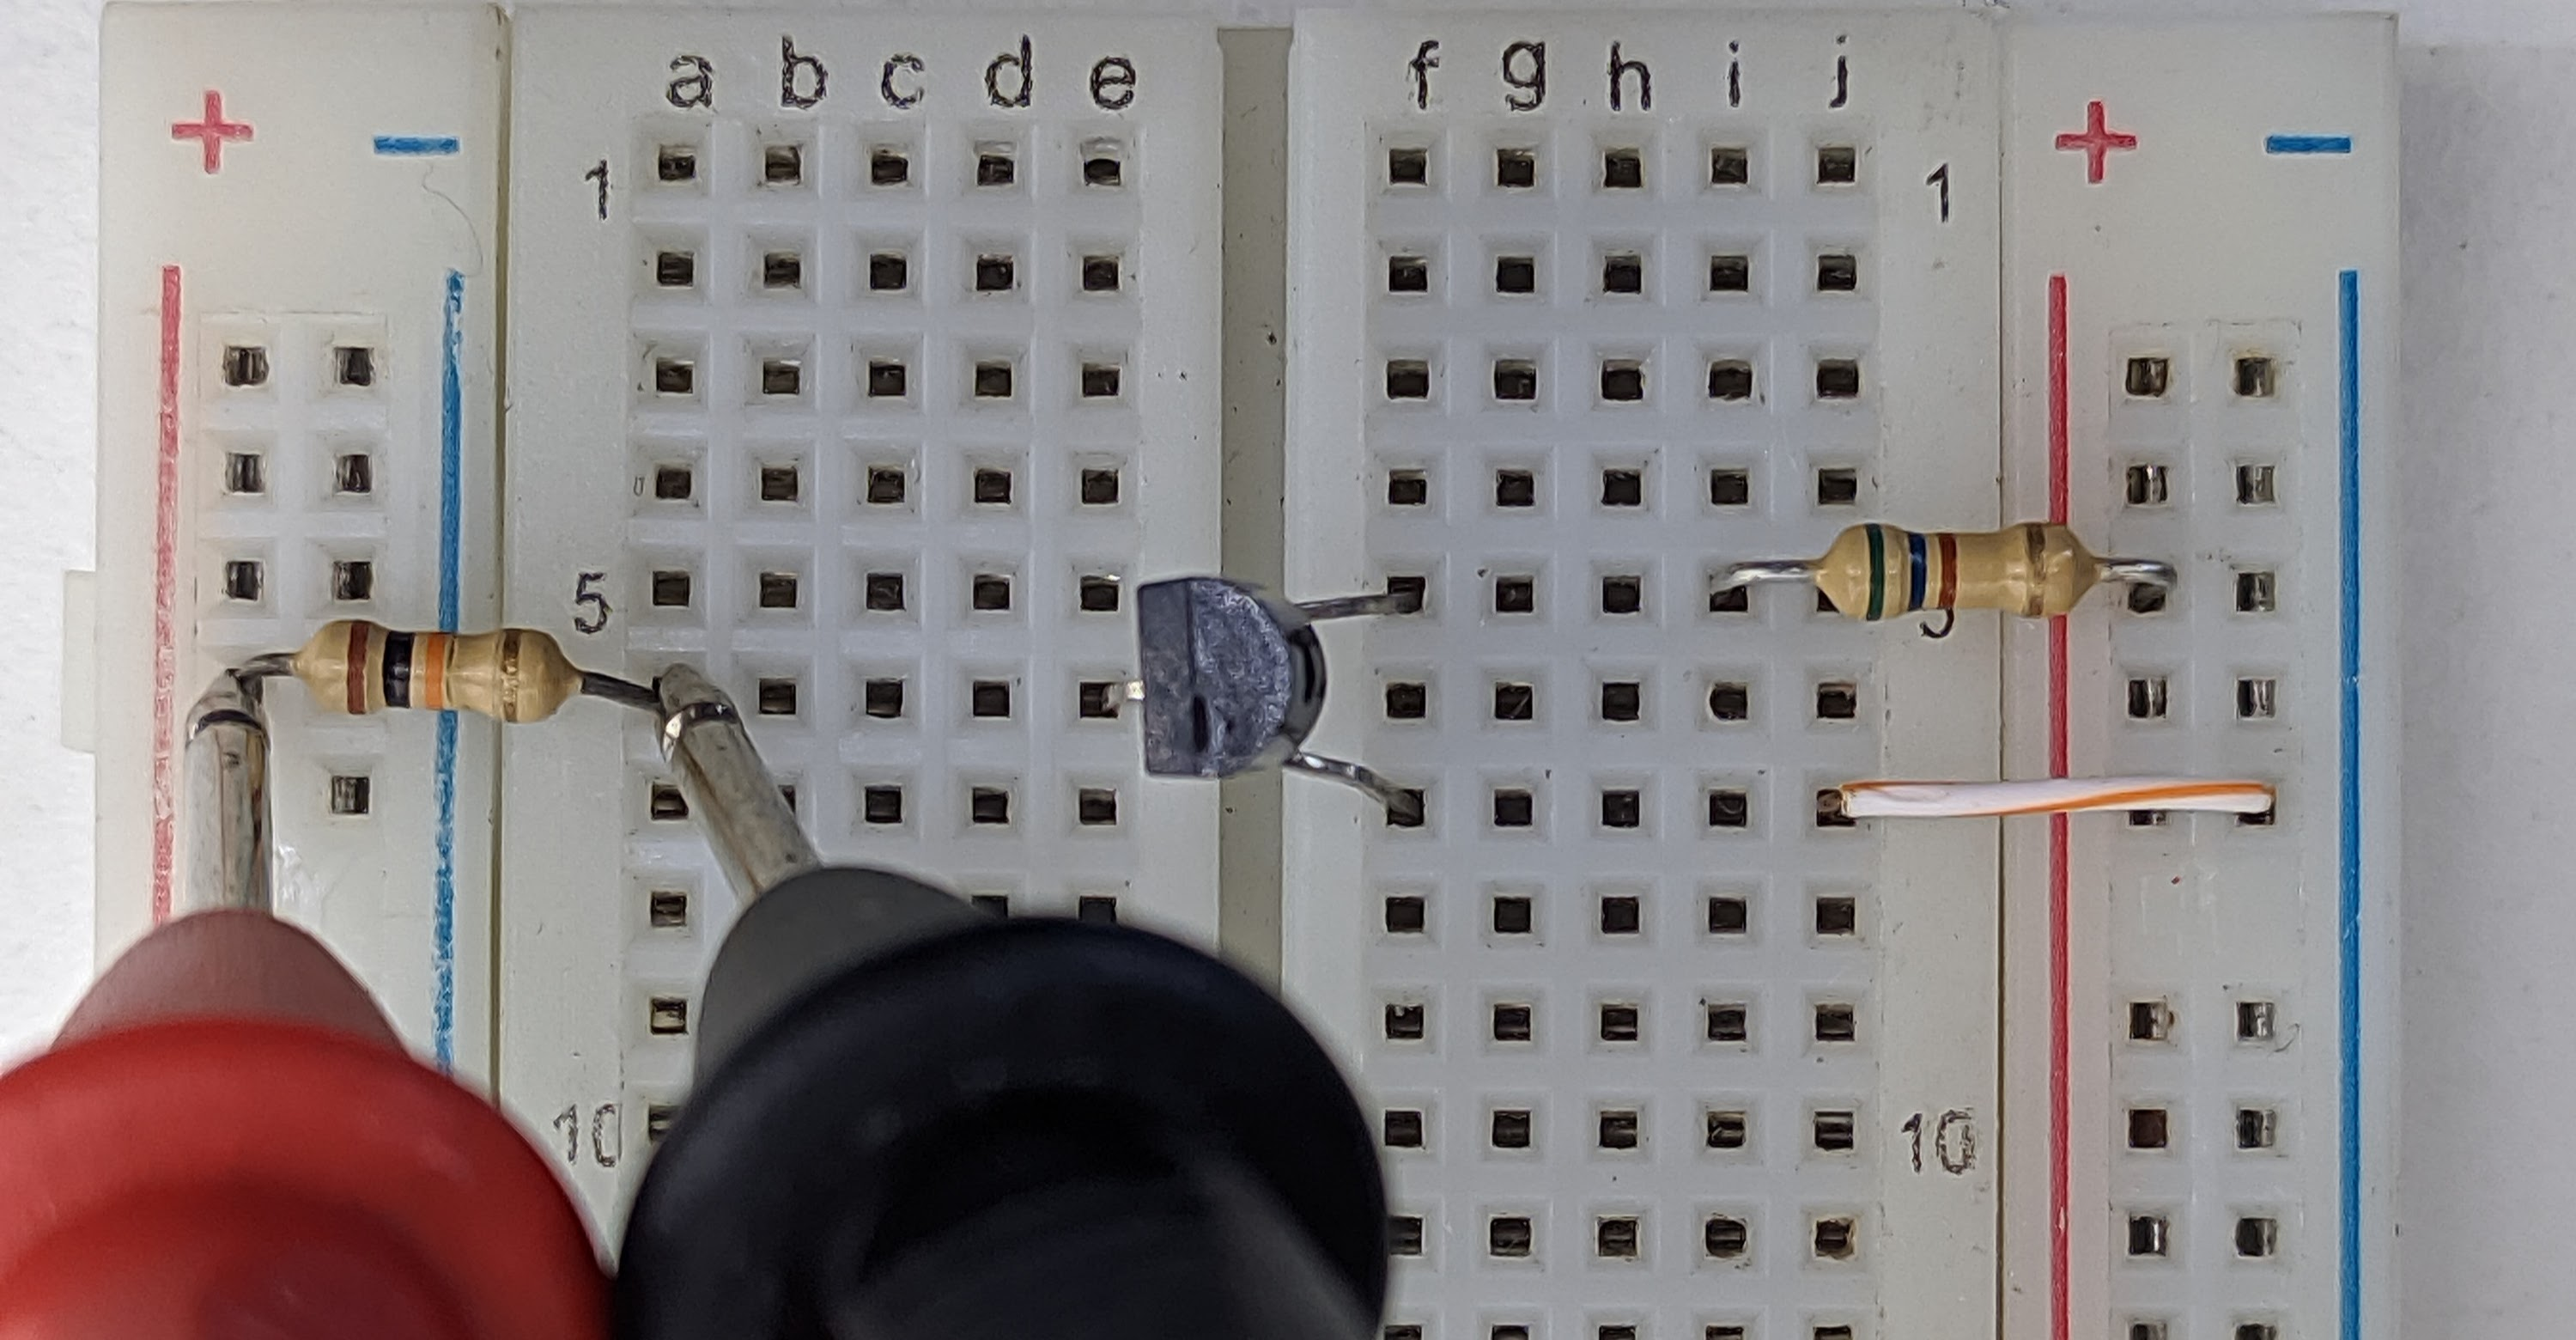
\includegraphics[width=1\textwidth]{tp3/pictures/prot_crkt-1_Vrb.jpg}
            \caption{Medicion de $V_{rb}$.}

        \end{minipage}    

        \begin{minipage}{0.25\textwidth}
        
            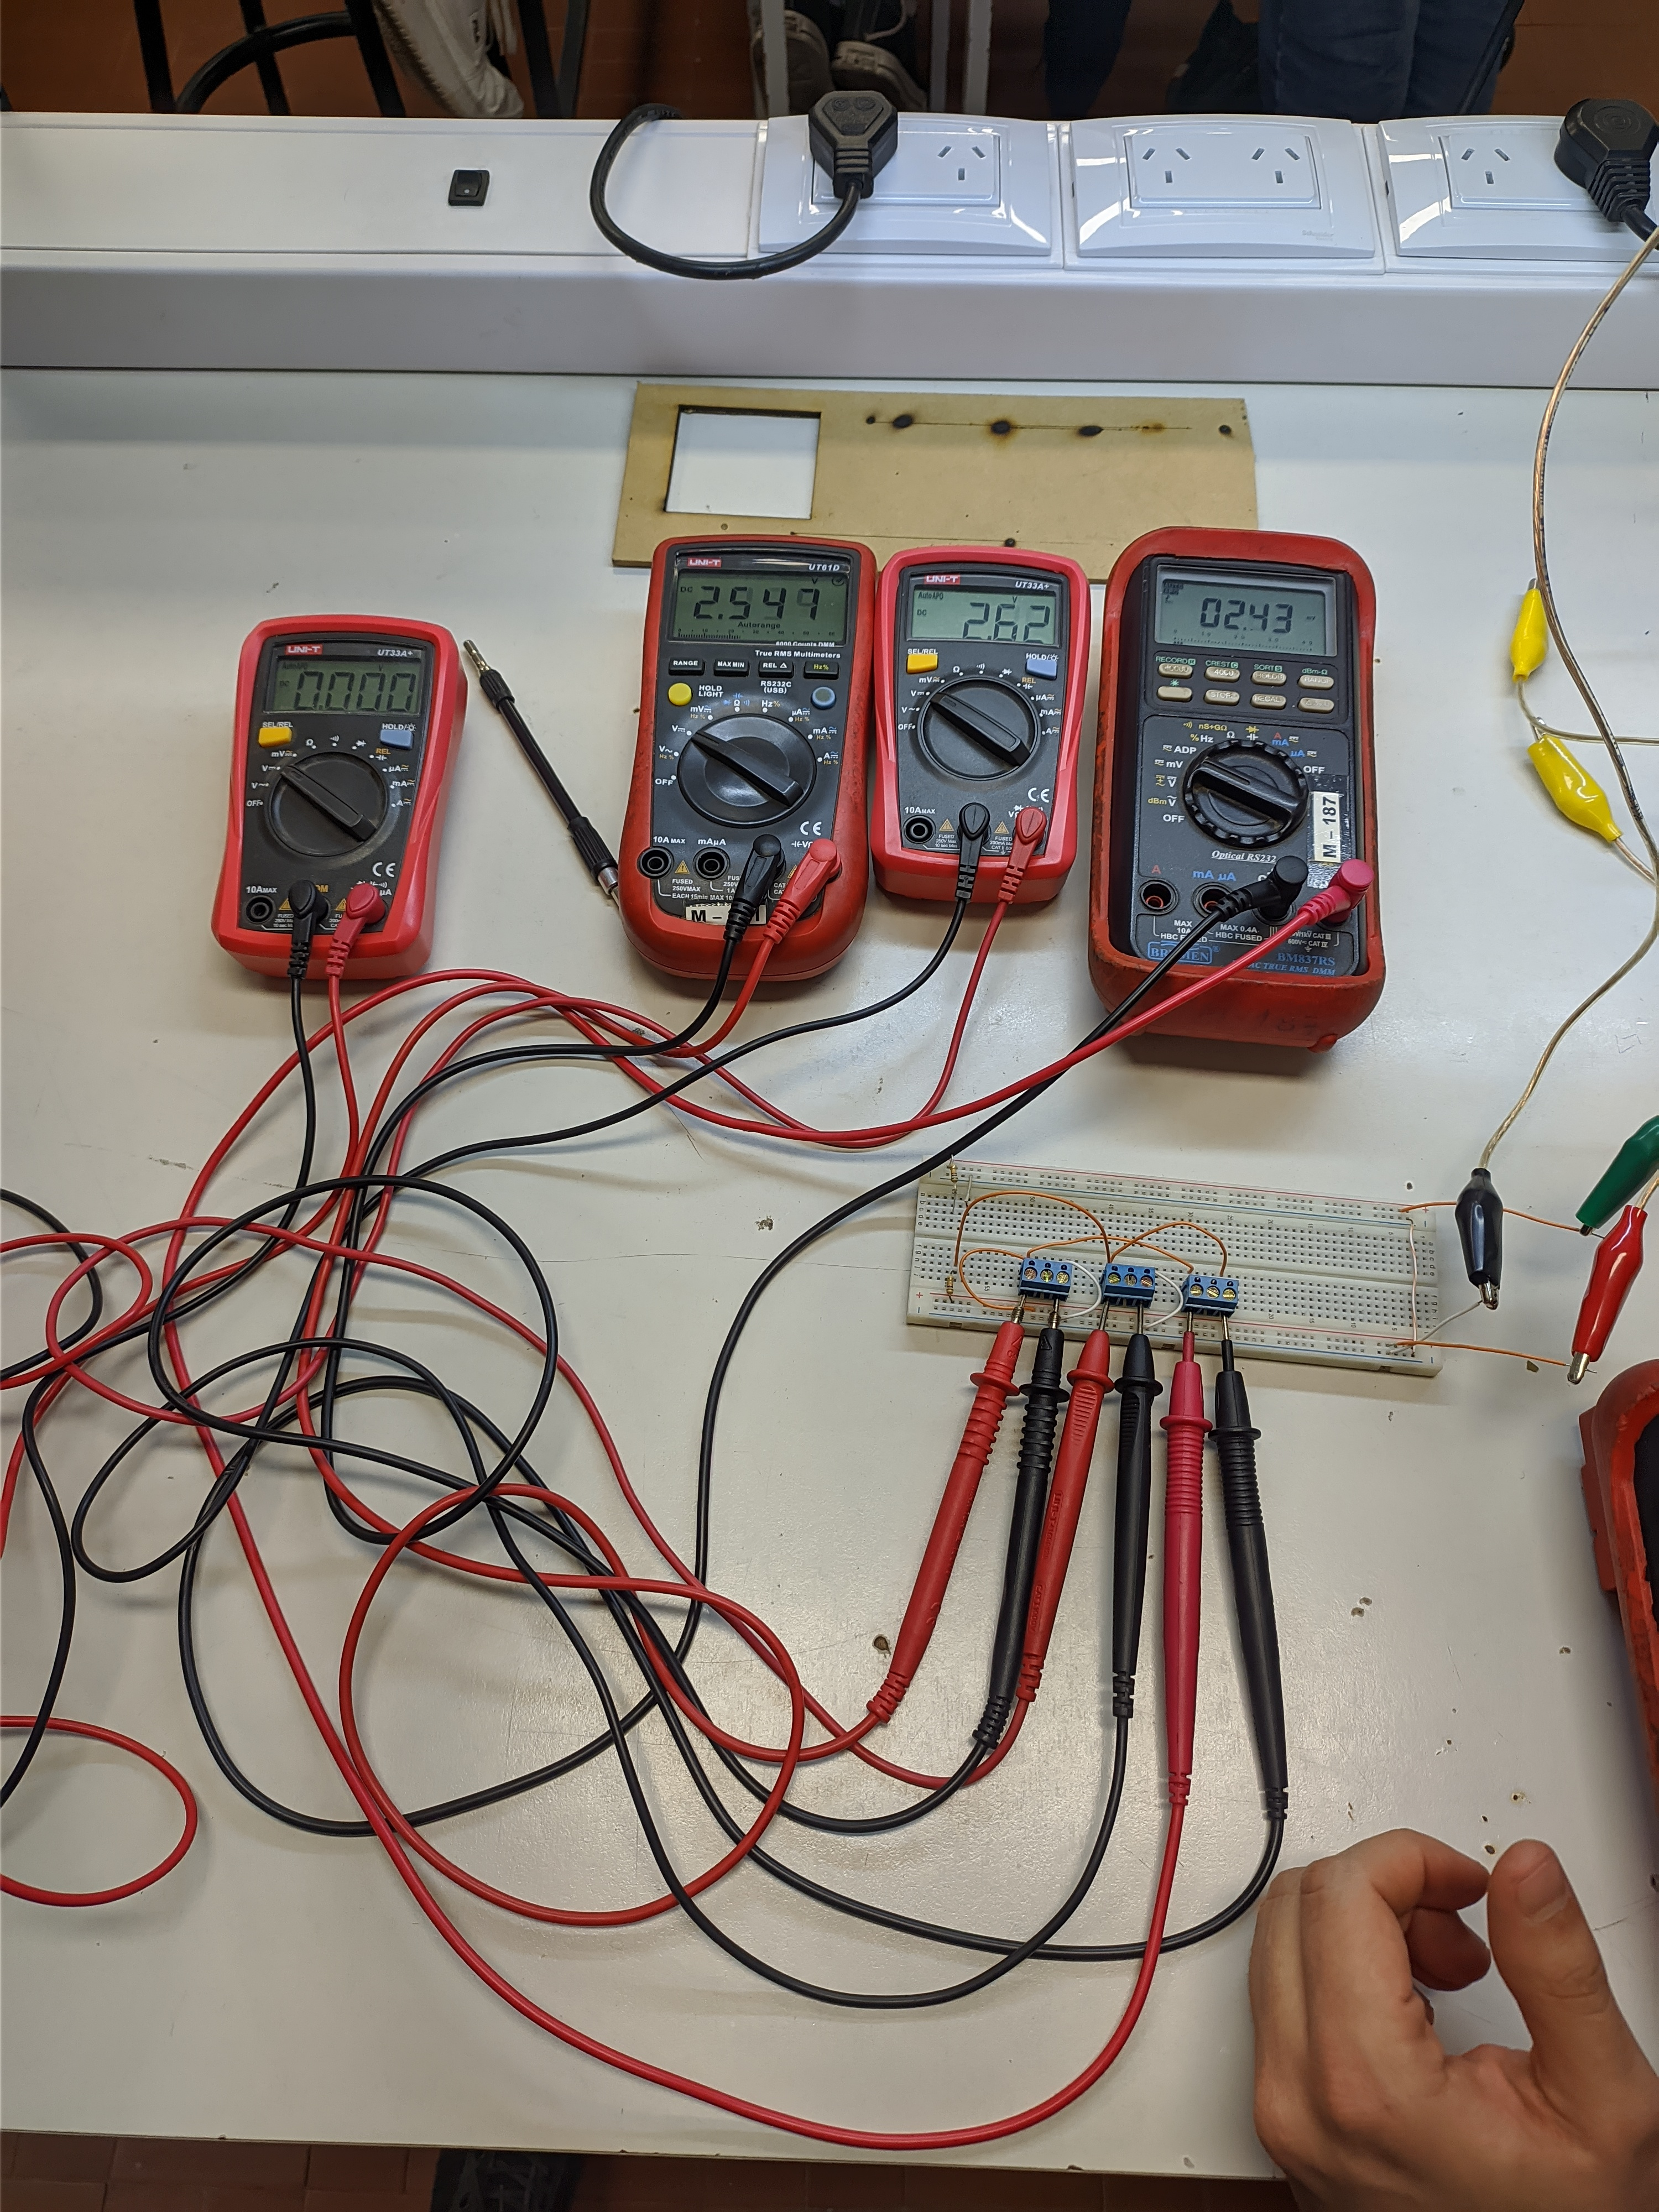
\includegraphics[width=1\textwidth]{tp3/pictures/setup_crkt-1.jpg}
            \caption{Posicion de las puntas para la medicion.}

        \end{minipage} 
        \end{center}
        
        

        
        
        
    \end{figure}


    Una vez se tiene preparado el circuito se prosigue a prender la fuente y ver como actua el transistor mientra aumentamos el voltaje $V_{BB}$ para asi obtener los datos para completar la tabla.


    Para completar la seccion de $I_B$ se realiza la siguiente formula:


    \begin{center}
        \[I_B=\frac{VBB-VBE}{RB}\]
    \end{center}






        
            \begin{table}[h!]
            \centering
            \resizebox{\textwidth}{!}{
            \begin{tabular}{|c|c|c|c|c|c|c|c|c|c|c|c|}
                \hline
                $V_{BB}$   & 0\,V & 300\,mV & 400\,mV & 500\,mV & 600\,mV & 700\,mV & 800\,mV & 1\,V & 3\,V & 7\,V & 10\,V \\
                \hline
                $I_B$      & 0\,A & -1.7\,µA & 0.5\,µA & 0.4\,µA & 0.9\,µA & 5.4\,µA & 18.6\,µA & 40\,nµA & 224.8\,µA & 0.623\,mA & 0.741\,mA \\
                \hline
                $V_{BE}$   & 0\,V & 317\,mV & 395\,mV & 496\,mV & 591\,mV & 646\,mV & 614\,mV & 600\,mV & 752\,mV & 765\,mV & 2.59\,V \\
                \hline
            \end{tabular}
            }
            \caption{Mediciones de $I_B$ y $V_{BE}$ para diferentes valores de $V_{BB}$. Valores de $I_B$ estimados según el comportamiento exponencial típico de la unión BE.}
        \end{table}




        \begin{figure}[h!]
            \centering
            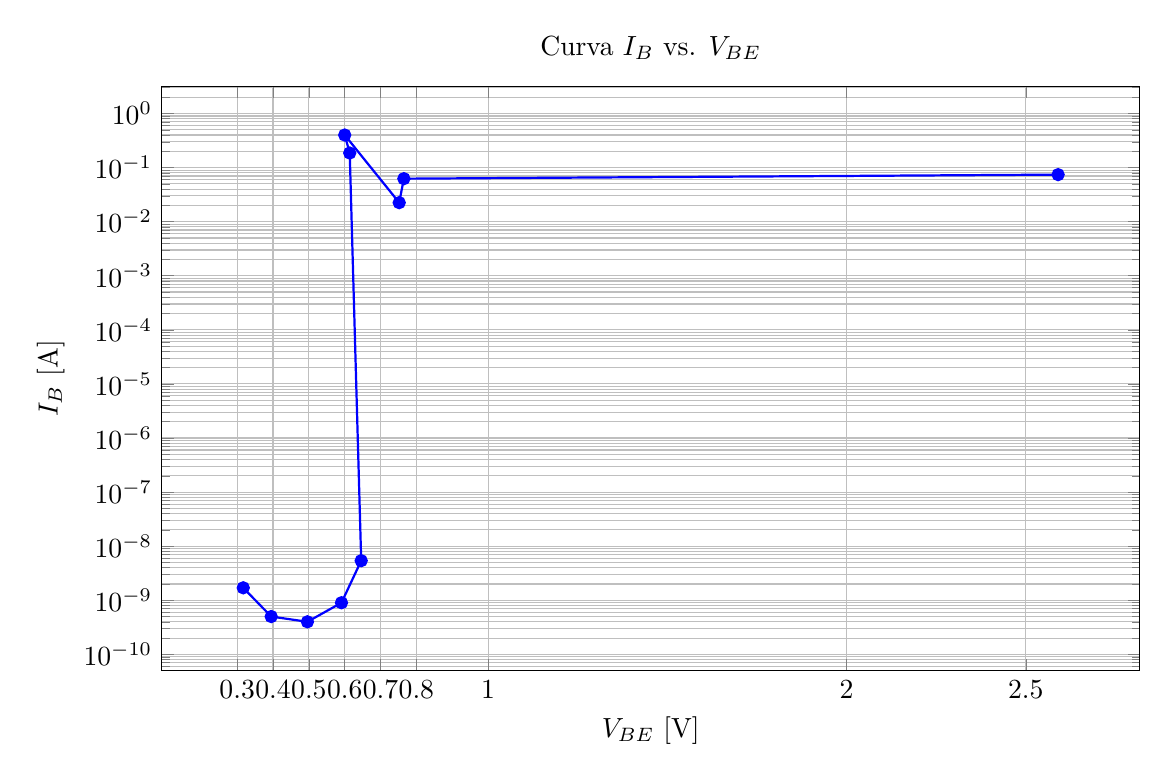
\begin{tikzpicture}
                \begin{axis}[
                        width=14cm,
                        height=9cm,
                        xlabel={$V_{BE}$ [V]},
                        ylabel={$I_B$ [A]},
                        ymode=log,
                        grid=both,
                        minor tick num=1,
                        log basis y=10,
                        title={Curva $I_B$ vs. $V_{BE}$},
                        xtick={0,0.3,0.4,0.5,0.6,0.7,0.8,1.0,2.0,2.5},
                        legend pos=north west
                    ]
                    \addplot[
                        mark=*,
                        color=blue,
                        thick
                    ]
                    coordinates {
                        (0.000, 0)
                        (0.317, 1.7e-9)
                        (0.395, 5.0e-10)
                        (0.496, 4.0e-10)
                        (0.591, 9.0e-10)
                        (0.646, 5.4e-9)
                        (0.614, 0.186)
                        (0.600, 0.400)
                        (0.752, 0.02248)
                        (0.765, 0.06235)
                        (2.59, 0.0741)
                    };
                \end{axis}
            \end{tikzpicture}
            \caption{Gráfico de la corriente de base $I_B$ en función de la tensión $V_{BE}$}
        \end{figure}
        
\newpage


    \section{Conclusion}


        En esta sección del trabajo práctico se analizaron las características de conducción de la juntura base-emisor del transistor BJT, considerando su comportamiento como una unión PN. A partir de mediciones experimentales, se observó que la tensión $V_{BE}$ necesaria para que comience la conducción se encuentra en el rango típico de los diodos de silicio, aproximadamente entre 0.6\,V y 0.7\,V.
        
        Se registraron valores de corriente de base $I_B$ para diferentes tensiones $V_{BB}$, verificando el crecimiento exponencial de $I_B$ en función de $V_{BE}$. Esta relación coincide con el modelo teórico de la ecuación del diodo, lo que confirma que el control de corriente en el BJT está fuertemente determinado por la polarización de esta juntura.
        
        Además, se destacó que pequeñas variaciones en $V_{BE}$ producen incrementos significativos en $I_B$, lo cual tiene un impacto directo en el control de la corriente de colector $I_C$ durante la operación en región activa. Estos resultados permiten comprender la importancia de la polarización adecuada de la base en el funcionamiento estable y eficiente del transistor.
